



\definecolor{cus_color}{rgb}{22, 96, 55}


\makeatletter
\newcommand{\removelatexerror}{\let\@latex@error\@gobble}
\makeatother


\begin{figure}[!t]
\centering
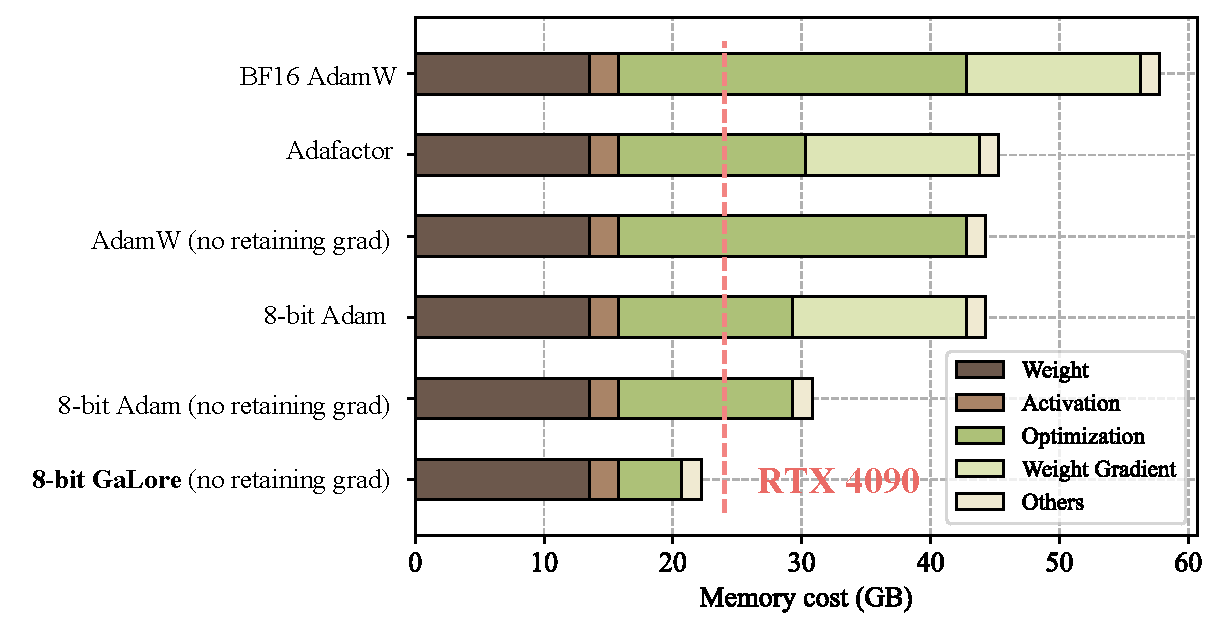
\includegraphics[width=1\columnwidth]{figures/files/memory_breakdown.pdf}
\vskip -0.11in
\caption{\small{Estimated memory consumption of pre-training a LLaMA 7B model with a token batch size of 256 on a single device, without activation checkpointing and memory offloading\protect\footnotemark[2]. Details refer to Section~\ref{sec:memory_measure}.}}
\label{fig:memory_breakdown} 
\vskip -0.15in
\end{figure}
\footnotetext[1]{The calculation is based on LLaMA architecture, BF16 numerical format, and maximum sequence length of 2048.}
\footnotetext[2]{In the figure, ``no retaining grad'' denotes the application of per-layer weight update to reduce memory consumption of storing weight gradient \citep{lvFullParameterFinetuning2023}.}
\SetAlFnt{\fontsize{8pt}{9pt}\selectfont}
\SetAlCapFnt{\fontsize{8pt}{9pt}\selectfont}
\begin{algorithm}[t]
    \SetAlgoLined
        \PyCode{for weight in model.parameters():} \\
        \Indp   %
            \PyCode{grad = weight.grad} \\ 
            \PyComment{original space -> compact space} \\
            \PyCode{lor\_grad = \textbf{project}(grad)} \\
            \PyComment{update by Adam, Adafactor, etc.} \\
            \PyCode{lor\_update = \textbf{update}(lor\_grad)} \\
            \PyComment{compact space -> original space} \\
            \PyCode{update = \textbf{project\_back}(lor\_update)} \\
            \PyCode{weight.data += update} \\
        \Indm %
    \caption{\fontsize{8pt}{9pt}\selectfont{\lowrank{}, PyTorch-like}}
    \label{alg:code_box}
\end{algorithm}
